\chapter{Experiential Learning of Networking Technologies: Understanding TCP Flow Control}

\begin{center}
{\large\uppercase{Ram P. Rustagi}}, 

(Department of CSE, KSIT Bengaluru) 

\vskip -6pt

\bigskip
{\large\uppercase{Viraj Kumar,}} 

(Divecha Centre for Climate Change, IISc Bengaluru)

\end{center}

\noindent\makebox[\textwidth]{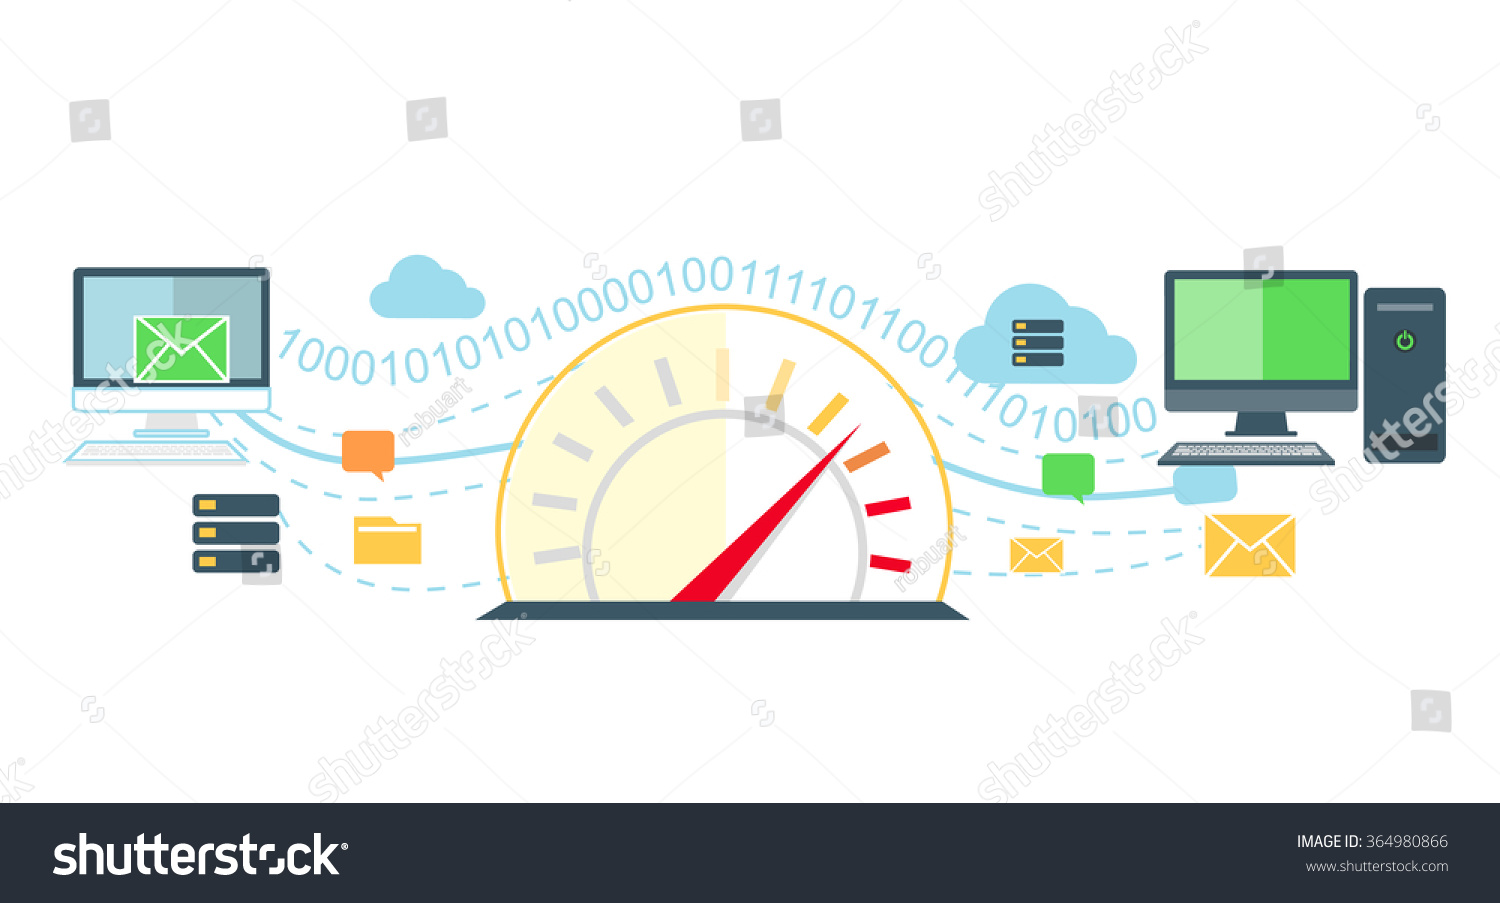
\includegraphics[width=1.05\paperwidth,height=13cm]{src/Figures/EL.jpg}}
\newpage

\begin{multicols}{2}

\section*{Abstract} 
In any TCP-based client-server communication, the application layer is implemented in the application program whereas the transport layer (i.e., TCP protocol) is implemented in the underlying operating system. TCP achieves reliability using acknowledgement packets and retransmitting any packets that are lost in the network, or corrupted, or delayed or delivered out-of-order. In addition, the TCP protocol ensures that the receiver application is not overwhelmed by data from the sender application – only the amount of data that the receiver can consume is transmitted. This is called TCP Flow Control. In this article, we explain the basics of flow control and provide experiential learning exercises to help understand its impact on TCP performance.

\section{Introduction}
In the last 3 articles \cite{art3-key04}\cite{art3-key05}\cite{art3-key06}, we have discussed scenarios of TCP communication and data transfer in general, TCP connection setup and tear down, and how TCP behaves under different network conditions. We have also defined various conditions that occur in the network, and ways to diagnose these conditions and address them. Once the TCP connection is setup and data transfer starts, the performance of TCP (in terms of throughput achieved) varies based on network conditions. In this article we will discuss Flow Control – an aspect of TCP behavior that influences data throughput in a connection.

When a TCP client (e.g. web browser) connects to a TCP server (e.g. web server), and a successful TCP connection is established between them, the client sends the request (URL) and the server sends the response (web page) back. When the response size is large (e.g., downloading a large file), the server (sender) would like to know the optimal rate at which it can send data to the client (receiver). If the server sends data at a higher rate than the receiver can receive and consume, overflow will occur at the receiver and excess data will be discarded. This would force the server to retransmit the data again. If the server sends the data at a lower rate, then it will take longer than necessary for the receiver to receive the entire data. Thus, both cases lead to sub-optimal performance. TCP protocol provides a mechanism for optimized delivery called flow control. In simple terms, flow control means that the receiver controls the rate at which the TCP sender sends the data. This rate is primarily determined by the size of the TCP buffer allocated at the receiver’s side. Whenever the receiver application issues read requests, the TCP stack supplies data to the application from this buffer, so the key question is: how large should this buffer be? When the receiver process requests the underlying operating system for a buffer, it risks allocating a buffer of sub-optimal size. If the allocated buffer size is too small, it will rapidly overflow: the receiver will be forced to discard these overflow packets, and the sender would be forced to wastefully resend these packets. If the allocated buffer size is too large, this may prevent other applications from running on the same host simply because resources have been allocated wastefully. Since a fixed buffer allocation strategy is problematic, the receiver needs to be flexible with its buffer allocation and dynamically change the buffer size in response to application characteristics as it consumes data over the TCP Connection. This aspect of TCP optimizes flow behavior. We now discuss the process by which the TCP protocol adjusts over time to achieve flow control.

\section{TCP Headers for Flow Control}

To enable TCP to implement flow control, the receiver informs the sender about the size of the buffer it has allocated during the connection setup. TCP supports this feature via its header field \textit{“receive window”}, a 16-bit long field at an offset of 14 bytes in the TCP header (Figure~\ref{chap3-fig01}). For a detailed understanding of TCP headers, the reader is directed to the TCP standard RFC 793 \cite{art3-key01}. With 16 bits, the maximum buffer size is just 64 KB. With today’s high-speed networks and easy availability of large memories, this 64 KB limit is far too restrictive and needs to be enhanced. This has been achieved by making use of the TCP Window Scale option \cite{art3-key02}\cite{art3-key03} which specifies a scaling factor by which the receive window size is multiplied. Thus, the maximum value of the TCP receive buffer can be as large as 1 GB \cite{art3-key02}\cite{art3-key03}.

The TCP protocol follows pipelined communications: the sender transmits one data segment after another without waiting for each ack, subject to the condition that total size of data segments sent is less than the receiver’s buffer size. Whenever the receiver receives a data segment, it sends an ack, which follows the process of cumulative acknowledgement\footnote{Cumulative acknowledgement means that when the ack value (3rd field in Figure~\ref{chap3-fig01}) is $N$, it implies that it has received all the data up to byte number $N – 1$. This implies that even if TCP segments containing ack values $N – k$ (for one or more values of $k \geq 1$) are lost, the ack value of $N$ in a subsequent packet implies all data up to byte $N – 1$ has, in fact, been received.}. Further, TCP is a streaming protocol and thus acknowledgement is at the byte-level and not at the segment-level. For a better understanding of TCP sequence number and acknowledgement number fields (fields 3 at offset of 4, and field 4 at offset of 8, the reader should refer to \cite{art3-key04}\cite{art3-key09}, where TCP streaming and reliability are discussed along with experiential learning exercises.
\setcounter{figure}{0}
\begin{figure}[H]
\centering
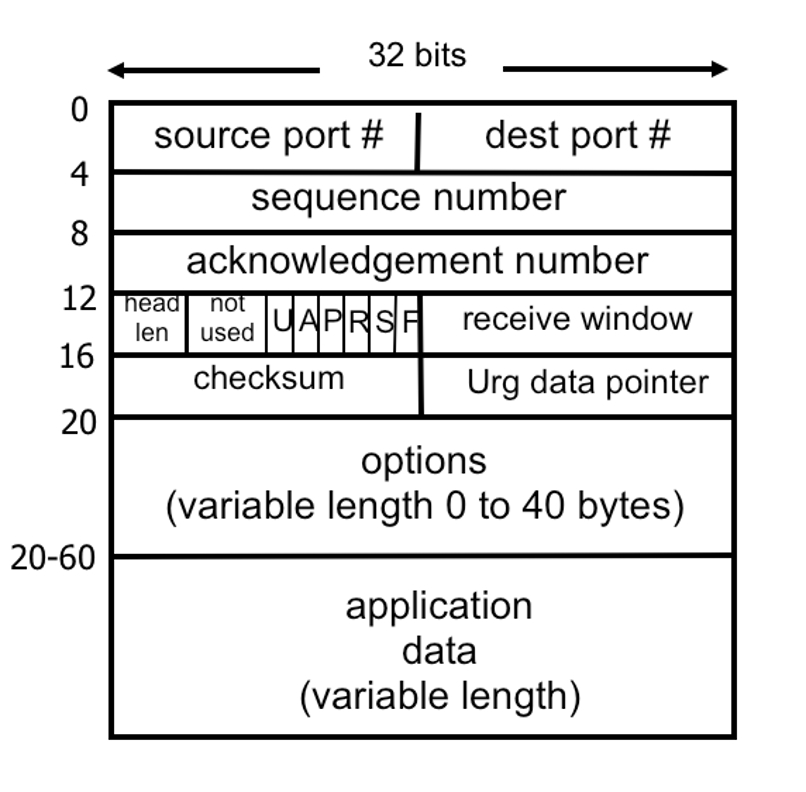
\includegraphics[scale=.95]{src/Figures/chap3/chap3-fig01.jpg}
\caption{TCP Headers}\label{chap3-fig01}
\end{figure}

\section{Basics of TCP Flow Control}

An excellent interactive resource for a basic understanding of flow control is available \cite{art3-key07}. For a more detailed understanding of its implementation using receive window buffer management, let us consider a scenario where the sender needs to transmit 10000 bytes of data. For simplicity, let us assume that the receiver has a buffer of size fixed at 4000 bytes (in reality, this buffer size is dynamically adjusted as per communication needs). Further, let us assume that the sender transmits 1000 bytes every 5 seconds whereas the receiver processes (consumes) 800 bytes every 8 seconds.

The status of the receive window size each time the sender transmits data and the receiver acknowledges the same is shown in Figure~\ref{chap3-fig02}. The following color coding has been used for ease of understanding: Black denotes TCP data transmitted by the sender, blue denotes TCP ack from the receiver, green denotes an update (decrease) in the rwnd (Receive Window) value when data is received from the sender and an ack is sent, and purple denotes an update (increase) in the rwnd value when the receiver application reads the buffer and thus makes some space available. (When rwnd = 4000–$k$, it means that $k$ bytes of data are already filled in the buffer and waiting for the application to read)

The sender first establishes a TCP connection with the receiver by performing a 3-way handshake (first 3 messages in Figure~\ref{chap3-fig02}) \cite{art3-key05}. The receiver informs the sender during the connection setup that its receive buffer size rwnd is 4000 bytes, as shown in Figure~\ref{chap3-fig02}. After the successful connection setup, the sender begins transmitting 1000 bytes of data every 5 seconds: ${\text{T}}_0, {\text{T}}_5, {\text{T}}_{10}, … $ etc. The TCP stack at the receiver sends the ack for each data segment by appropriately updating its rwnd value to indicate the memory available in the receiver’s buffer for this connection. 
\begin{figure}[H]
\centering
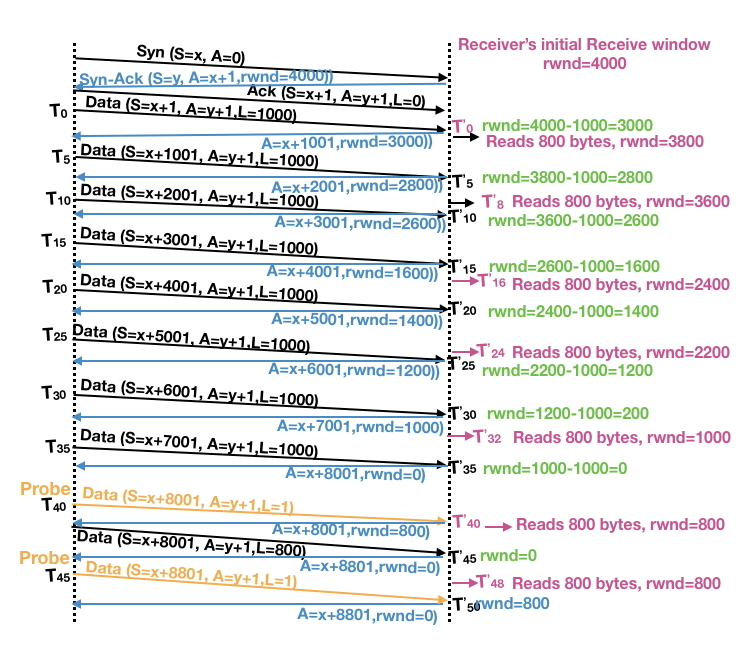
\includegraphics[scale=1.4]{src/Figures/chap3/chap3-fig02.jpg}
\caption{ Adjustment of receive window at receiver}\label{chap3-fig02}
\end{figure}

During the connection setup, the sender is informed that the receiver can receive up to 4000 bytes of data at a time. Thus, at time ${\text{T}}_0$, the sender transmits 1000 bytes as it can transmit up to 4000 bytes. The receiver receives this data at time ${\text{T’}}_{0}$ (slightly after ${\text{T}}_{0}$, because of transmission delay and propagation delay \cite{art3-key08}), stores it in the buffer and updates rwnd to 3000 (4000 - 1000). This updated value is communicated to the sender via the ack. Since the application at the receiver is waiting for data that is now available, it immediately reads 800 bytes from the TCP buffer and starts processing it. This frees 800 bytes from the buffer and hence rwnd is updated to 3800 (3000 + 800). Note that 200 bytes of data are still in the buffer, waiting to be read by the application. At time ${\text{T}}_5$, the sender transmits the next 1000 bytes of data. Once again, the receiver stores this data in the buffer and returns the updated value of rwnd = 2800 (3800-1000) to the sender via the ack. This pattern continues, with the value of rwnd eventually decreasing to 0 after the sender transmits 1000 bytes at ${\text{T}}_{35}$.

\section{Zero Window Probe}

At this point $({\text{T}}_{35})$, the sender cannot transmit any more data since it has received an ack with rwnd=0, indicating that the receiver’s buffer is full. In the scenario we are considering, the application will read 800 bytes from the receiver’s buffer and update rwnd to 800. However, the receiver cannot send a duplicate ack (this can lead to other implications on TCP connections). Thus, both the sender and the receiver appear to be stuck. This deadlocked scenario is generally known as “TCP Zero Window” \cite{art3-key10}\cite{art3-key11}, and it can lead to severe performance issues. Exercise~\ref{chap3-Exe3} describes an experiment to better understand this phenomenon.

Fortunately, TCP provides a mechanism to deal with Zero Window: the sender can periodically transmit a Zero Window Probe (ZWP) message, which could be as small as a single byte of data. Once the receiver gets this TCP message from the sender, it must respond with an ack. Thus, if a ZWP is received after rwnd has been updated to a positive number, the receiver can indicate to the sender that its buffer is no longer full in the ack. Two ZWPs are shown in yellow in Figure~\ref{chap3-fig02}. The first of these probes is initiated at time ${\text{T}}_{40}$. If we assume that the application clears 800 bytes from the reader’s buffer before this probe arrives at time ${\text{T}}_{40}$, the resulting ack will indicate a positive rwnd value – as shown here. In contrast, consider the second probe initiated at time ${\text{T}}_{45}$. In this case, there still isn’t any free space in the reader’s buffer and hence the ack reports that the value of rwnd is still 0. One or more additional ZWPs (not shown) would have to be issued before data transmission can continue.

ZWPs are used in many other networking applications. For example, consider a network printer that prints documents sent from the machines it is connected to. Since the printer has no data to send, it is the receiver. Suppose that the printer runs out of paper and it takes several minutes to replenish the paper stock. During this interval, the printer may continue to receive documents (without actually printing anything) until its buffer is full. In this case, it will send an ack with the value of rwnd = 0 to the sender machine. This machine can periodically send ZWPs to the printer, and as soon as the paper stock has been replenished, it will resume printing by consuming the data from the receiver buffer. At this point, the value of rwnd will become greater than zero and the ack for subsequent ZWPs will indicate that the printer is ready to receive new documents.

Alert readers may have noticed a potential problem with this seemingly neat mechanism: an adversary can launch a Denial of Service (DoS) attack \cite{art3-key11} by opening connections to a server (sender) and immediately responding with rwnd = 0. This would force the server to waste resources by sending ZWPs (the attacker would respond to each ZWP with rwnd = 0), thus creating a DoS attack. To thwart such attacks, the server follows the standard TCP exponential backoff mechanism where the interval between successive ZWPs doubles each time, up to a pre-configured maximum number of retries. If this limited number of retries is exhausted, the TCP connection may be closed prematurely, releasing resources and avoiding DoS attacks. We now describe a real-life instance where this issue occurred while the first author of this article was managing the cloud deployment of servers.

In this scenario, end users needed to download the roughly 2.5 GB Android image of a mobile phone over a 2 Mbps to 4 Mbps link. In contrast, the servers were interconnected via a Gigabit Ethernet network, as shown in Figure~\ref{chap3-fig03}. User connections terminated at the Load Balancer (LB), and the LB would initiate a new connection to the Web Server (WS). The WS, in turn, would connect with the Application Server (AS) and Data Store (DS). Thus, for a single download interaction for end-user $U$, the LB would be dealing with two TCP Connections: a connection ${\text{TCP}}_{U}$ where the LB was the sender and $U$ was the receiver, and a connection ${\text{TCP}}_{WS}$, where the WS was the sender and the LB was the receiver. When the download was initiated, the WS could pump data at a very high rate over ${\text{TCP}}_{WS}$, whereas data was consumed by the user $U$ at a far lower rate over ${\text{TCP}}_{U}$.
\begin{figure}[H]
\centering
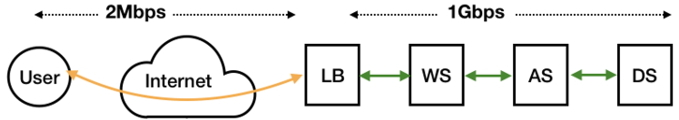
\includegraphics[scale=1.55]{src/Figures/chap3/chap3-fig03.jpg}
\caption{Schematic describing a real-life issue due to TCP Zero Window}\label{chap3-fig03}
\end{figure}

\vskip -.4cm

In order to store as much data as possible from the WS, the LB was forced to rapidly increase its receiver buffer size for ${\text{TCP}}_{WS}$ (by requesting more memory from the OS) until it reached its maximum. This buffer was emptied by copying to the buffer for ${\text{TCP}}_U$, but this occurred at a very slow rate. Due to the huge bandwidth available for ${\text{TCP}}_{WS}$, the WS received an rwnd value of 0 from the LB even after multiple ZWPs. When the retry threshold was exceeded, the connection ${\text{TCP}}_{WS}$ was terminated with about 0.4 GB unsent to the LB. Thus, the end-user was unable to download the entire image.

When this problem was reported in the field, the engineering team responded, as it should by proposing probable causes, based on prior experience and the available data. Suspicion initially fell on the AS application, and when no fault was discovered, the analysis proceeded further. Eventually, and only because of a clear understanding of the TCP Zero Window issue, the problem was diagnosed correctly. (If the first author’s role with the team had not ended shortly after this, the next task would have been to examine strategies for fixing the issue – such as reconfiguring the maximum number of ZWP retries and/or timeout values – and rank these based on the available resources.)

For an experiential understanding of TCP Flow control, reader should follow the steps as defined in Exercise~\ref{chap3-Exe1} and Exercise~\ref{chap3-Exe2}.

\section{Summary}

TCP flow control ensures that the receiver is not overwhelmed by data from the sender. In contrast, the User Datagram Protocol (UDP) does \textit{not} support flow control. Over a UDP connection, the receiver can become overwhelmed and will be forced to drop some of the transmitted data.

Flow control is one of the two key mechanisms that govern TCP performance – the other mechanism is Congestion Control. We will examine Congestion Control in detail in the next article, but briefly it is a mechanism that allows the sender to discover a near-optimal rate at which data can be transmitted over the TCP connection, keeping in mind that network capacity can vary significantly over the course of the data transmission. If the sender transmits data at an excessively low rate, it will be under-utilizing the network capacity and will take more than the optimal time to transmit the entire data. On the other hand, if it sends data at a higher rate than what network can sustain, it will choke the network. As a result, packets will queue up in the network at various stages when buffers become full, some packets will be dropped by intermediate network devices, such as routers, and this will lead to higher queuing delay and wasteful retransmission of packets.

Even though both congestion control and flow control deal with different error conditions, they have the same objective of improving TCP performance and the response of the TCP implementation in both these error conditions is the same – retransmit lost/corrupted/discarded/delayed data segments. Thus, a common misconception is to consider these as equivalent conditions. However, as we shall see in the next article, they are quite different and should be understood differently.

\section{Experiential Exercises}

All the exercise steps described assume that two machines, namely, Client (C\_m) and Server (S\_m) are connected via a network. An example of this connectivity is shown in Figure~\ref{chap3-fig04}. The client machine C\_m is an Ubuntu Linux and server machine could be any machine (Ubuntu/MacOS/Windows) etc. To understand the flow control behavior, two simple Python programs (to be run with python3) are provided: one for the client \url{(accs_client.py)}, which will connect to the server and simply receive data, and the other for the server \url{(accs_server.py)}, which will accept connection from the client and send data. These programs are listed in the Appendix.
\begin{figure}[H]
\centering
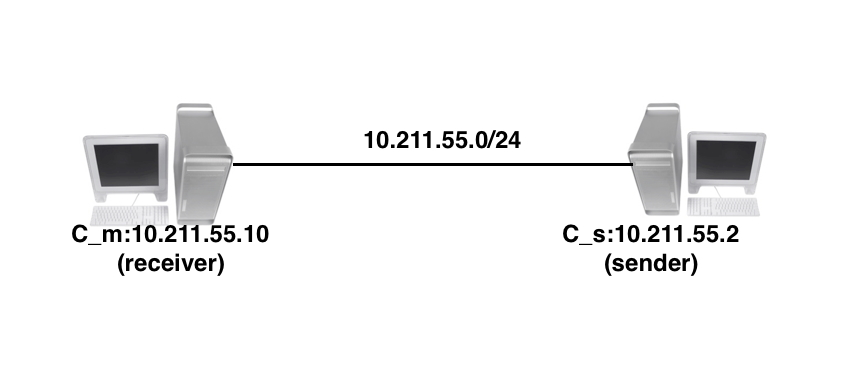
\includegraphics[scale=1.4]{src/Figures/chap3/chap3-fig04.jpg}
\caption{ Basic setup for experiential learning}\label{chap3-fig04}
\end{figure}

\setcounter{section}{0}
\section{Exercise}\label{chap3-Exe1}

\textbf{Topic: Basic understanding of TCP Flow Control with default setup i.e. with Window Scaling}
\begin{itemize}
\item[a.] On the server machine, run the server program as 

\texttt{python3  accs\_server.py -b 200 -d 1 -p 9999}

This will wait for one client to connect and send 200 bytes of data every second.

\item[b.] On the client machine, in one terminal run tcpdump program to look at the window size which is sent. Tcpdump program is used with basic default option and it will show the receive window value (the value of rwnd).  Use the port number 9999 (or any other port of your choice) to capture the traffic. Assuming that the server’s IP address is 10.211.55.2 and uses port number 9999, invoke the command as below

\texttt{sudo tcpdump -n -i enp0s5 host 10.211.55.2 and port 9999}

Please check the Ethernet interface name and replace it appropriately instead of enp0s5.

\item[c.] On the client machine, in another terminal, invoke the client program which will read 100 bytes at a time at an interval of 2 seconds, as below

\texttt{python3 accs\_client.py -s 10.211.55.2 -p 9999 -b 100 -d 2 -c 1000}

Please check the IP address of server and replace it appropriately instead of 10.211.55.2.

\item[d.] The above will connect to the server, and the server will start sending data, which will be displayed on screen.

\item[e.] Look at the output of tcpdump command (in step 2 above), and look at the window size. Note down the value of \texttt{win field} and it is likely to increase with each packet received from server. Given below are sample output for first 4 capture outputs of packets sent from client to server. Notice that \texttt{win field} value starts increasing slowly. The value of ack field is consecutively as 201, 401, 601 etc. i.e. increases by 200 each time indicating that 200 bytes are received. Since data is continuously received, TCP stack slowly increases the client receive buffer size as well.

20:09:21.091424 IP 10.211.55.10.60892 $>$\\
10.211.55.2.9999: Flags [.], ack 201, win 237, options [nop,nop,TS val 1385669 ecr 780230225], length 0

20:09:22.093950 IP 10.211.55.10.60892 $>$\\ 10.211.55.2.9999: Flags [.], ack 401, win 245, options [nop,nop,TS val 1385919 ecr 780231222], length 0

20:09:23.095784 IP 10.211.55.10.60892 $>$\\ 10.211.55.2.9999: Flags [.], ack 601, win 254, options [nop,nop,TS val 1386170 ecr 780232218], length 0

20:09:24.098482 IP 10.211.55.10.60892 $>$\\ 10.211.55.2.9999: Flags [.], ack 801, win 262, options [nop,nop,TS val 1386420 ecr 780233215], length 0

\item[f.] Both the client and server programs are flexible in terms of buffer size (option –b) and delay interval (option –d) and readers are requested to carry the exercise with different values of these options to develop a better understanding of TCP Flow control.
\end{itemize}


\section{Exercise}\label{chap3-Exe2}

\textbf{Topic: TCP Flow Control with Window Scaling disabled.}
\begin{itemize}
\item[a.] On the client machine (Ubuntu), note down the default values (or currently configured) of TCP window scaling and receiver buffer size. Use the following commands to obtain the values.

\texttt{\$ sudo sysctl net.ipv4.tcp\_window\_scaling}

\texttt{ net.ipv4.tcp\_window\_scaling = 1 }
 
 \texttt{\$ sudo sysctl  net.ipv4.tcp\_rmem }
 
 \texttt{net.ipv4.tcp\_rmem = 4096	87380	6291456}
 
 The default value of Window Scaling is 1 implying Window scaling is supported and we will set it to zero to disable the scaling. Similarly, \texttt{\url{net.ipv4.tcp\_rmem}}  provides 3 set of value, first one corresponds to minimum, $2^{\text{nd}}$ one corresponds to default buffer allocation, and last one the max values. Please make a note of these values so as to restore these back after the exercise is completed, otherwise machine may provide poor performance for any TCP connection. For a simple implementation to understand TCP Flow control, set all these values as 4096. Use the following commands to disable the window scaling and receive buffer size. 
 
 \texttt{\$ sudo sysctl-w net.ipv4.tcp\_window\_scaling=0}
 
\texttt{net.ipv4.tcp\_window\_scaling = 0}

\texttt{\$ sudo sysctl -w net.ipv4.tcp\_rmem="4096 4096 4096"}

\texttt{net.ipv4.tcp\_rmem = 4096 4096 4096}

\texttt{\$ sudo sysctl net.ipv4.tcp\_window\_scaling}

\texttt{net.ipv4.tcp\_window\_scaling = 0}

\texttt{\$ sudo sysctl  net.ipv4.tcp\_rmem}

\texttt{net.ipv4.tcp\_rmem = 4096	4096	4096}

These TCP Tuning parameters are set only temporarily and if machine is booted, TCP will start with its default value.

 \item[b.] Repeat the steps of exercise~\ref{chap3-Exe1} i.e. run the server and client program respectively and also observe the value of \texttt{win field} in tcpdump.

\item[c.] As TCP Window scaling is disabled, the rwnd starts from value of 1460 (corresponding to 1500 bytes of Ethernet payload minus 20 bytes of IP header minus 20 bytes of TCP header), and decreases by 200 in each ack packet since data packet contains 200 bytes. A sample dump of tcpdump command for the packets sent from client to server are given below. Thus, the rwnd value starts decreasing from 1460 (initial) to 1260, then 1060, then to 860 and so on. The client program is also reading the data, but at delayed intervals and in smaller amounts, so the read buffer will fill up. You will notice the value remains at 860 for a while (on account of client read as well as some intricate implementations of TCP), and then after a while it starts decreasing again to 660, 460 etc.

21:09:48.598063 IP 10.211.55.10.60904 $>$\\ 10.211.55.2.9999: Flags [.], ack 201, win 1260, options [nop,nop,TS val 1912572 ecr 782330922], length 0

21:09:49.600109 IP 10.211.55.10.60904 $>$\\ 10.211.55.2.9999: Flags [.], ack 401, win 1060, options [nop,nop,TS val 1912823 ecr 782331920], length 0

21:09:50.601628 IP 10.211.55.10.60904 $>$\\ 10.211.55.2.9999: Flags [.], ack 601, win 860, options [nop,nop,TS val 1913073 ecr 782332919], length 0

21:09:51.603529 IP 10.211.55.10.60904 $>$\\ 10.211.55.2.9999: Flags [.], ack 801, win 860, options [nop,nop,TS val 1913323 ecr 782333919], length 0

21:09:52.608485 IP 10.211.55.10.60904 $>$\\ 10.211.55.2.9999: Flags [.], ack 1001, win 860, options [nop,nop,TS val 1913575 ecr 782334920], length 0

21:09:53.610785 IP 10.211.55.10.60904 $>$\\ 10.211.55.2.9999: Flags [.], ack 1201, win 860, options [nop,nop,TS val 1913825 ecr 782335921], length 0

21:09:54.615655 IP 10.211.55.10.60904 $>$\\ 10.211.55.2.9999: Flags [.], ack 1401, win 860, options [nop,nop,TS val 1914076 ecr 782336923], length 0

21:09:55.620261 IP 10.211.55.10.60904 $>$\\ 10.211.55.2.9999: Flags [.], ack 1601, win 660, options [nop,nop,TS val 1914328 ecr 782337926], length 0

21:09:56.622550 IP 10.211.55.10.60904 $>$\\ 10.211.55.2.9999: Flags [.], ack 1801, win 460, options [nop,nop,TS val 1914578 ecr 782338926], length 0
\end{itemize}


\section{Exercise}\label{chap3-Exe3}

\textbf{Topic: TCP Zero Window Probe.}
\begin{itemize}
\item[a.]  Repeat the steps of exercise~\ref{chap3-Exe2} and observe the value of \texttt{win field} for a while. A sample output of TCP exchange between server and client is given below when rwnd becomes zero. This happens after about 12 seconds when 2600 bytes of data have been sent from the server. 

21:19:49.301804 IP 10.211.55.10.60910 $>$\\ 10.211.55.2.9999: Flags [.], ack 1, win 1460, options [nop,nop,TS val 2056798 ecr 782906007], length 0

21:19:49.302448 IP 10.211.55.2.9999 $>$\\ 10.211.55.10.60910: Flags [P.], seq 1:201, ack 1, win 65535, options [nop,nop,TS val 782906007 ecr 2056798], length 200

21:19:49.302484 IP 10.211.55.10.60910 $>$\\ 10.211.55.2.9999: Flags [.], ack 201, win 1260, options [nop,nop,TS val 2056798 ecr 782906007], length 0

:\\
:\\
:

21:20:01.334506 IP 10.211.55.10.60910 $>$\\ 10.211.55.2.9999: Flags [.], ack 2601, win 136, options [nop,nop,TS val 2059806 ecr 782917978], length 0

21:20:07.387763 IP 10.211.55.2.9999 $>$\\ 10.211.55.10.60910: Flags [.], seq 2601:2737, ack 1, win 65535, options [nop,nop,TS val 782923999 ecr 2059806], length 136

21:20:07.387809 IP 10.211.55.10.60910 $>$\\ 10.211.55.2.9999: Flags [.], ack 2737, \underline{\textbf{win 0}}, options [nop,nop,TS val 2061320 ecr 782923999], length 0

21:20:12.494967 IP 10.211.55.2.9999 $>$\\ 10.211.55.10.60910: Flags [.], seq 2737:2738, ack 1, win 65535, options [nop,nop,TS val 782929083 ecr 2061320], \underline{\textbf{length 1}}

21:20:12.495002 IP 10.211.55.10.60910 $>$\\ 10.211.55.2.9999: Flags [.], ack 2737, \underline{\textbf{win 0}}, options [nop,nop,TS val 2062596 ecr 782929083], length 0

21:20:17.900971 IP 10.211.55.2.9999 $>$\\ 10.211.55.10.60910: Flags [.], seq 2737:2738, ack 1, win 65535, options [nop,nop,TS val 782934455 ecr 2062596], \underline{\textbf{length 1}}

21:20:17.901014 IP 10.211.55.10.60910 $>$\\ 10.211.55.2.9999: Flags [.], ack 2737, \underline{\textbf{win 0}}, options [nop,nop,TS val 2063948 ecr 782934455], length 0


\item[b.] In the $6^{\text {th}}$ packet in above display (in actual there will be few more packets which have not been shown here for brevity), from client to server, the value of win field is 0 (shown as underlined and in bold) implying that receiver buffer has become full.

\item[c.] In the subsequent packet ($7^{\text {th}}$), which is from server to client, it is a probe packet as can be determined from length value of 1 (shown in bold and underline).

\item[d.] In response to Zero Window Probe, client still responds with win=0 ($8^{\text{th}}$ packet) as its receive buffer is still full. 

The above explains the phenomenon of Zero Window Probe. Please restore the value of TCP window scaling and memory allocation for receive buffer to its system default value by using the following command (or even performing a reboot).

\texttt{\$ sudo sysctl -w net.ipv4.tcp\_window\_scaling=1}

\texttt{\$ net.ipv4.tcp\_window\_scaling = 0}

\texttt{\$ sudo sysctl -w net.ipv4.tcp\_rmem=" 4096 87380 6291456"}

\texttt{net.ipv4.tcp\_rmem = 4096 87380 6291456}
\end{itemize}

\section*{Appendix}
{\lstset{xleftmargin=1cm}
{\bf Client program: accs\_client.py.}\\
{\bf \#--------------------------------------------------------------------------------}
\begin{lstlisting}[language=Caml,basicstyle=\small]
#!/usr/bin/python3
import socket
import time
import argparse

parser = argparse.ArgumentParser
	(description=
	 "Simple Server for N/w Delays")
parser.add_argument('-s', '--server', 
		type=str, required=True)
parser.add_argument('-p', '--port', 
		type=int, default=9999)
parser.add_argument('-c', '--count', 
		type=int, default=10)
parser.add_argument('-d', '--delay', 
		type=int, default=5)
parser.add_argument('-b', '--buffer', 
		type=int, default=50)
args = parser.parse_args()

ip_addr = args.server
port = args.port
count = args.count
delay = args.delay
buffer = args.buffer

srvr_addr = (ip_addr, port)
sock = socket.socket(socket.AF_INET, 
		socket.SOCK_STREAM)
sock.connect(srvr_addr)

for i in range(1,count):
    data = sock.recv(buffer)
    print ("received:", data)
    time.sleep(delay)

sock.close()
\end{lstlisting}}
{\bf \#--------------------------------------------------------------------------------}

\bigskip

{\bf Server program: accs\_server.py.}\\
{\bf \#--------------------------------------------------------------------------------}

\begin{lstlisting}[language=Caml,basicstyle=\small]
#!/usr/bin/python3
import socket
import time
import argparse

parser = argparse.ArgumentParser
	(description=
	 "Simple Server for N/w Delays")
parser.add_argument('-s', '--server', 
		type=str, default="0.0.0.0")
parser.add_argument('-p', '--port', 
		type=int, default=9999)
parser.add_argument('-d', '--delay',  
		type=int, default=1)
parser.add_argument('-b', '--buffer',  
		type=int, default=100)
args = parser.parse_args()

ip_addr = args.server
port = args.port
delay = args.delay
buffer = args.buffer

sock = socket.socket(socket.AF_INET, 
		socket.SOCK_STREAM)
srvr_addr = (ip_addr, port)
sock.bind(srvr_addr)
sock.listen(5)
connsock, client = sock.accept()
print("received a conn from", str(client))

while True:
    msg = "A" * buffer
    print ("Sending:", msg)
    sent = connsock.send(msg.encode('ascii'))
    time.sleep(delay)
\end{lstlisting}
{\bf \#--------------------------------------------------------------------------------}\hfill \raisebox{-.1cm}{\includegraphics[scale=.9]{src/Figures/circledC.eps}}

\begin{thebibliography}{99}
\bibitem{art3-key01}RFC 793, “Transmission Control Protocol “, Information Sciences Institute, USC, CA, Sep 1981,

 \url{https://tools.ietf.org/html/rfc793.} Last accessed May 2019.

\bibitem{art3-key02}  RFC 1323, “TCP extensions for Long Delay Paths “, Jacobson, Braden, Oct 1988 

\url{https://tools.ietf.org/html/rfc1072}, Last accessed May 2019.

\bibitem{art3-key03} RFC 7323, “TCP extensions for High Performance“, Borman, Braden, Jacobson, Scheffenegger, Oct 1988 

\url{https://tools.ietf.org/html/rfc7323#page-8}, Last accessed May 2019.

\bibitem{art3-key04} Ram Rustagi, Viraj Kumar, “Understanding Transport Layer Basics”, ACCS journal of Computing and Communications, Vol 2, Issue 3, Sep 2018. 

\url{https://acc.digital/experiential-learning-of-networking-technologies-understanding-transport-layer-basics/}, last accessed Nov 2018.

\bibitem{art3-key05}Ram Rustagi, Viraj Kumar, “Understanding TCP States- Part I”, ACCS journal of Computing and Communications, Vol 2, Issue 4, Dec 2018 

\url{https://acc.digital/experiential-learning-of-networking-technologies-understanding-tcp-states-part-1/}, last accessed May 2019

\bibitem{art3-key06}Ram Rustagi, Viraj Kumar, “Understanding TCP States- Part I”, ACCS journal of Computing and Communications, Vol 3, Issue 1, Mar 2019

 \url{https://acc.digital/experiential-learning-of-networking-technologies-understanding-tcp-states-part-2/}, last accessed June 2019

\bibitem{art3-key07} Understanding TCP Flow control with interactive animations,

 \url{https://media.pearsoncmg.com/aw/ecs_kurose_compnetwork_7/cw/content/interactiveanimations/flow-control/index.html}, last accessed May 2019.

\bibitem{art3-key08} Ram Rustagi, Viraj Kumar, “Understanding Network Delays”, ACCS journal of Computing and Communications, Vol 1, Issue 3, Dec 2017;  

\url{https://acc.digital/experiential-learning-of-networking-technologies-understanding-network-delays/}, last accessed Nov 2018.

\bibitem{art3-key09} Kurose, Ross, “Computer Networking: A Top Down Approach”, section 3.5.5, $6^{\text{th}}$ edition, Pearson, 

\bibitem{art3-key10}RFC 1122, “Requirements for Internet Hosts -- Communication Layer”, Braden, IETF, Oct 1989. 

\url{https://tools.ietf.org/html/rfc1122}, Last accessed June 2019.

\bibitem{art3-key11} RFC 6429, “TCP Sender Clarification for Persist Conditions”, Bashyam, Jethanandani, Ramaiah, Dec 2011, 

\url{https://tools.ietf.org/html/rfc6429}, last accessed June 2019.

\end{thebibliography}
\end{multicols}



\noindent
\begin{tabular}{V{2.5}cp{14cm}V{2.5}}
\clineB{1-2}{2.5}
 &\\
\raisebox{-4cm}{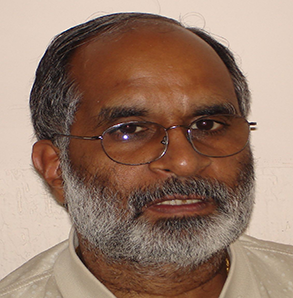
\includegraphics{src/Figures/authors/Rustagi_RPR-PP-Photo.png}} & 

\centerline{\large\bf Prof. Ram P. Rustagi}

\bigskip
Dr. Ram P. Rustagi is currently working as Professor, CSE dept, KSIT Bangalore, and honed up his academic skills with Ph.D from IIT Delhi, and M.Tech from IISc Bangalore. Prior to KSIT, at Cavisson Systems, he mentored new technology development using Machine Learning techniques in Security and Performance Monitoring. At PES University, he had taught Undergraduates, Post Graduates students, and successfully guided 3 Ph.D scholars. At PESU, he brought innovations in teaching computer network and security courses, and introduced practical experiential learning exercises.\\
&\\  
\raisebox{-3.7cm}{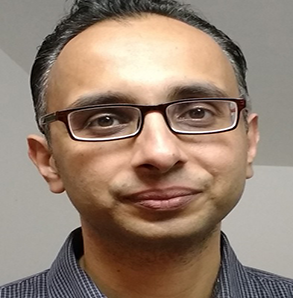
\includegraphics{src/Figures/authors/Viraj_Kumar.png}} & 

\centerline{\large\bf Prof. Viraj Kumar}

\bigskip
Dr. Viraj Kumar is a Visiting Professor at the Divecha Centre for Climate Change, IISc Bangalore and the Vice-Chair of ACM India’s Special Interest Group in Computer Science Education (iSIGCSE). He was a consultant to the Committee to draft the National Education Policy (2017-18), and contributed to two education-related task groups of the Karnataka Knowledge Commission (2014-16). He holds a PhD in Computer Science from the University of Illinois at Urbana-Champaign.\\
&\\
\clineB{1-2}{2.5}
\end{tabular}

\begin{figure}[H]
\centering

\includegraphics[scale=.15]{src/Figures/QR-codes/qr-code_experiential-learning.png}

\medskip

{\large\sf Access this article on the Web}
\end{figure}

